\documentclass[12pt]{article}
\usepackage{natbib}
\usepackage[french]{babel}
\usepackage[T1]{fontenc}
\usepackage{url}
\usepackage[utf8x]{inputenc}
\usepackage{amsmath}
\usepackage{mathtools}
\usepackage{graphicx}
\graphicspath{{images/}}
\usepackage{parskip}
\usepackage{amssymb}
\usepackage{xurl}
\usepackage{caption}
\usepackage{geometry}
\geometry{hmargin = 2.5cm, vmargin = 2.5cm}

\title{Modèle de Percolation}							% Title
\date{\today}											% Date

\makeatletter
\let\thetitle\@title
\let\theauthor\@author
\let\thedate\@date
\makeatother

\begin{document}
%%%%%%%%%%%%%%%%%%%%%%%%%%%%%%%%%%%%%%%%%%%%%%%%%%%%%%%%%%%%%%%%%%%%%%%%%%%%%%%%%%%%%%%%%

\begin{titlepage}
	\centering
    
\includegraphics[scale = 0.7]{University.png}\\[1.0 cm]	% University Logo
    \textsc{\LARGE \newline\newline Faculté des Sciences appliquées}\\	% University Name
	\textsc{\Large  INFO0902-1 : Structures de données et algorithmes}\\[0.5 cm]				% Course Code
	\rule{\linewidth}{0.2 mm} \\[0.4 cm]
	{ \huge \bfseries \thetitle}\\
	\rule{\linewidth}{0.2 mm} \\[2 cm]
	
	\begin{minipage}{0.5\textwidth}
		\begin{flushleft} \large
			\emph{Professeur:}\\
			GEURTS Pierre\\
			\end{flushleft}
			\end{minipage}~
			\begin{minipage}{0.4\textwidth}
            
			\begin{flushright} \large
			\emph{Groupe:} \\
			LAMBERMONT Romain\\
            LOUIS Arthur\\
		\end{flushright}
        
	\end{minipage}\\[5 cm]
	
	
    \thedate
	
\end{titlepage}

%%%%%%%%%%%%%%%%%%%%%%%%%%%%%%%%%%%%%%%%%%%%%%%%%%%%%%%%%%%%%%%%%%%%%%%%%%%%%%%%%%%%%%%%%
\thispagestyle{empty}
\tableofcontents
\listoffigures
\pagebreak
\setcounter{page}{1}

\section{Analyse Théorique}

\subsection{Description \texttt{UnionFindTree.c}}
Dans le cadre de ce projet nous avons réalisé une structure d'UnionFind utilisant le principe de \textit{Path Compression}, 
qui permet de réduire la profondeur de l'arbre à chaque appel de la fonction \texttt{ufFind}. Ce principe réduit considérablement
le temps d'accès à un ensemble et d'union à un autre par la fonction \texttt{ufUnion}.

\subsection{Complexités \texttt{ufUnion} et \texttt{ufFind}}

Pour l'implémentation par liste liée, nous avons gardé dans la structure de chaque noeud un pointeur vers sa liste. 
De plus, lors de l'union de deux ensembles, nous ajoutons toujours le plus court ensemble au plus long ensemble 
grâce à un champ de la structure liste qui garde à jour le nombre d'éléments que possède la liste.
Pour cette implémentation, l'opération \texttt{ufFind} est $\mathcal{O} (1)$ quoi qu'il arrive et
\texttt{ufUnion} est dans le pire des cas $\mathcal{O}(n/2)$ et dans le meilleur des cas, elle est $\Omega(1)$.

En ce qui concerne l'implémentation par arbre, nous avons gardé dans la structure de chaque noeud un pointeur vers son parent direct. 
Nous avons profité des opérations \texttt{ufFind} pour procéder à une \textit{Path Compression} 
et lors des \texttt{ufUnion}, nous relions le plus petit arbre au grand, c'est la \textit{Fusion Optimisée des Racines}.
Cela permet de réduire le nombre d'opérations nécessaires pour atteindre la racine du plus petit arbre.
Cela permet de diminuer la profondeur de l'arbre 
et donc de réduire le temps de calcul pour le prochain appel à la fonction \texttt{ufFind}. 
Pour cette implémentation, la complexité dans le pire des cas de \texttt{ufFind} est $\mathcal{O} (n)$ 
mais cela est compensé par la path compression
qui fait en sort que ce cas ne se présente jamais dans la pratique 
et dans le meilleur des cas, elle est  $\mathcal{O} (1)$. 
Pour finir, l'implémentation de \texttt{ufUnion} est dans le pire des cas $\mathcal{O}(n/2)$ et dans le meilleur des cas $\Omega (1)$.
\paragraph{}
Voici les sources utilisée pour répondre à cette question :

\begin{itemize}
	\item \url{https://stackoverflow.com/questions/53149097/why-is-the-time-complexity-of-performing-n-union-find-union-by-size-operations}
	\item \url{https://fr.wikipedia.org/wiki/Union-find}
	\item \url{https://algorithms.tutorialhorizon.com/disjoint-set-union-find-algorithm-union-by-rank-and-path-compression/}
\end{itemize}

\subsection{Structure \texttt{Percolation.c}}
Pour notre structure percolation, nous avons fait le choix de travailler avec trois champs : une size, qui contient la taille de la grille 
(size $\times$ size), une matrice de booléens (type ajouté par le librairie \texttt{stdbool.h}) qui détermine si une case est ouverte ou fermée 
(\texttt{false} = case fermée, \texttt{true} = case ouverte) et un \texttt{UnionFind} qui permettera de réaliser les opérations \texttt{ufUnion} et \texttt{ufFind}.
\paragraph{}
Nous allons maintenant vérifier que les fonctions de l'interface de \texttt{Percolation.c} respectent bien les conditions demandées :
\begin{itemize}
	\item \texttt{percCreate} : Cette fonction réalise $n + 3$ allocations de mémoire pour la structure et $2n$ appels à une fonction de l'interface d'\texttt{UnionFind}
	\item \texttt{percFree} : Cette fonction réalise $n$ appels à la matrice de booléens et trois appels constants à la structure
	\item \texttt{percSize} : Cette fonction réalise un seul appel à la structure
	\item \texttt{percOpenCell} : Cette fonction réalise des appels constants à la structure et des appels à des fonctions de l'interface d'\texttt{UnionFind}
	\item \texttt{percIsCellOpen} : Cette fonction réalise un seul appel à la structure
	\item \texttt{percIsCellFull} : Cette fonction réalise un seul appel à la structure et deux appels à des fonctions de l'interface d'\texttt{UnionFind}
	\item \texttt{percPercolates} : Cette fonction réalise deux appels à la structure et deux appels à des fonctions de l'interface d'\texttt{UnionFind}
	\item \texttt{percPrint} : Vérification non nécessaire
\end{itemize}
\vspace{0.5cm}
On vérifie bien que les conditions sont respectées.

\subsection{Complexité en temps et espace de \texttt{thresholdEstimate} par listes}
Lorsque nous réalisons $T$ percolations pour une grille de $N \times N$ items et que nous ouvrons $m$ cellule, la complexité en temps dans le pire des cas peut s'écrire : \[\mathcal{O}(T\times(N^2 + N + m \times (k+N/2)))\] 
où $k$ est le nombre de coordonnées alétoires nécessaires pour trouver une cellule fermée.

La complexité en espace peut s'écrire : \[ N^2 + T + \log{T}\]
Le $\log{T}$ est du au \texttt{QuickSort} du tableau des résultats.

\subsection{Complexité en temps et espace de \texttt{thresholdEstimate} par arbres}

Lorsque nous réalisons $T$ percolations pour une grille de $N \times N$ items et que nous ouvrons $m$ cellule, 
la complexité en temps dans le pire des cas peut s'écrire : \[\mathcal{O}(T \times (N^2 + N + m \times (k+\frac{3 \times N}{2})))\] où $k$ 
est le nombre de coordonnées alétoires nécessaires pour trouver une cellule fermée.
\\La complexité en espace est la même qu'au cas précédent.

\newpage
\section{Analyse Empirique}

\subsection{Centilles et seuil critique de percolation}

\begin{figure}[!h]
    \centering
	\captionsetup{justification = centering}
    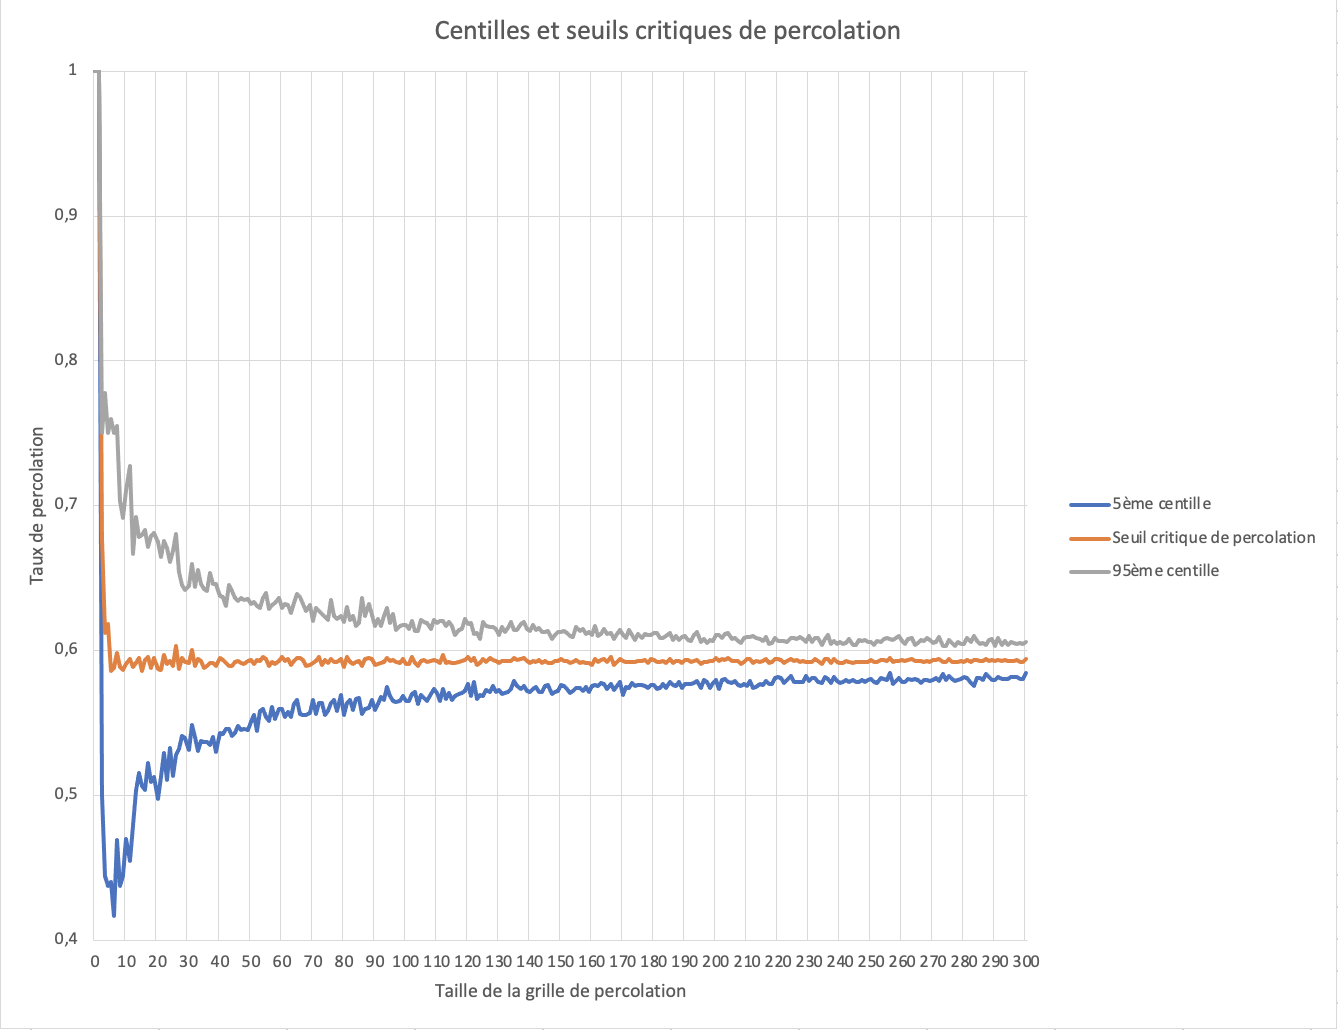
\includegraphics[scale = 0.3]{Centilles.png}
    \caption{Graphique des centilles et seuils critiques de percolation en fonction de la taille de la grille}
    \label{fig:centilles_taux}
\end{figure}

En observant ces courbes, on remarque qu'au départ, avec une taille de grille $1 \times 1$, les valeurs du tableau de résultats, 
représenatant dans l'ordre les 5èmes centilles, le seuil critique de percolation et les 95èmes centilles, que les trois valeurs démarrent
logiquement toutes à la valeur $1$, en effet une grille $1 \times 1$ percole forcément. 
\\
En augmentant la taille, dans notre cas, jusque 
$300 \times 300$, on remarque très logiquement que la courbe des 5èmes et 95èmes centilles se retrouvent respectivement au-dessus et en-dessous de 
la courbe de seuil critique de percolation tout en convergeant vers celle-ci. En observant la courbe de seuil, on se rend compte que cette valeur 
tend vers $59\%$, valeur plutôt logique.
\subsection{Temps d'exécution en fonction de l'implémentation}
\begin{figure}[!h]
    \centering
	\captionsetup{justification = centering}
    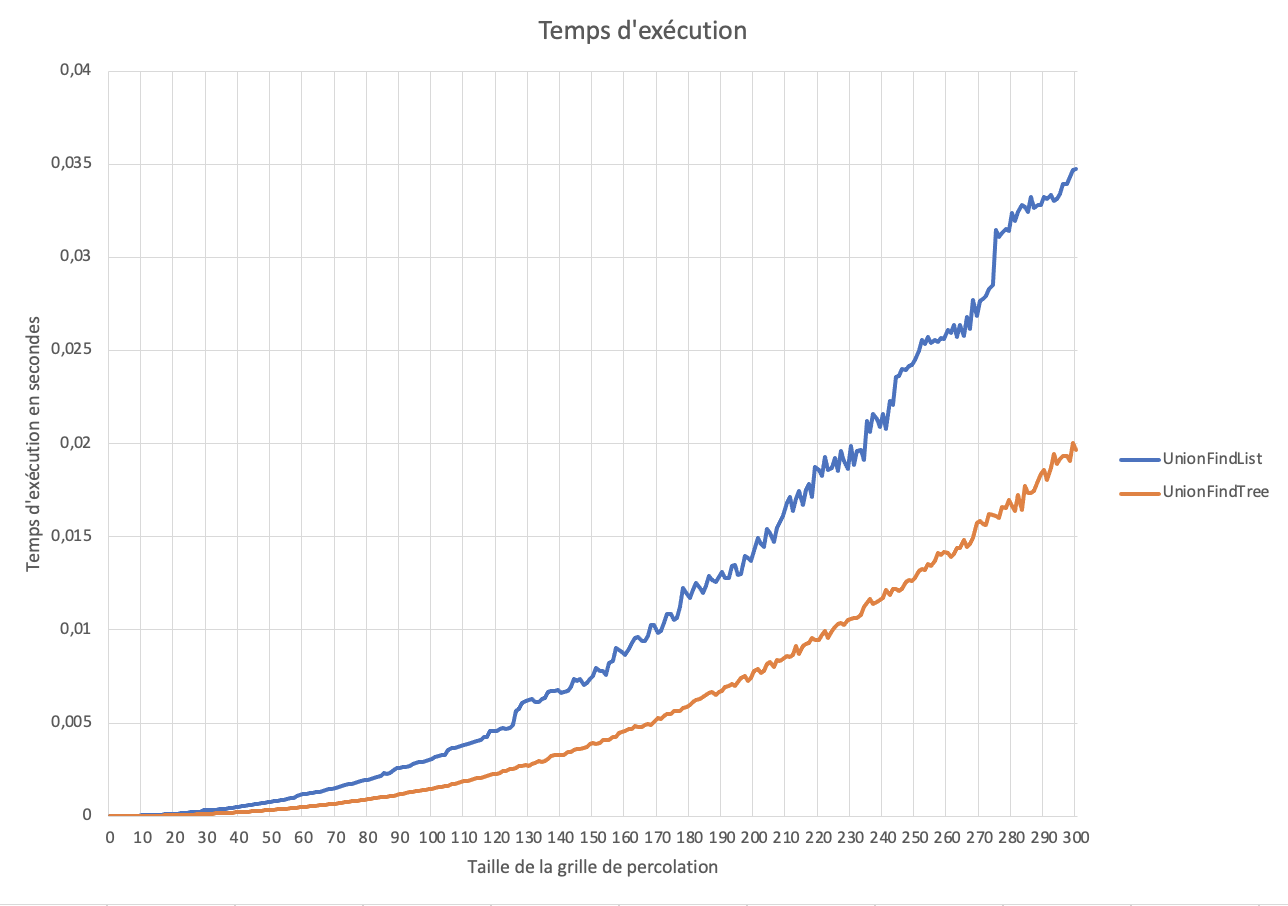
\includegraphics[scale = 0.3]{Temps.png}
    \caption{Graphique des temps d'exécution en fonction de la méthode d'implémentation et de la taille de la grille}
    \label{fig:my_label}
\end{figure}
En observant le graphique obtenu ci-dessus, on remarque que pour des petites grilles (jusque $40 \times 40$), les temps de calculs 
sont fort similaires et ce pour une bonne, raison. Les amélioration du \textit{Path Compression} et de la \textit{Fusion Optimisée des Racines} n'ont pas encore eu le temps de se démarquer par rapport 
à la fonction \texttt{UnionFindList.c}. Par après, les deux courbes se séparent car le \texttt{ufFind} de l'implémentation sous forme de liste devient alors plus lent et moins efficace.
\subsection{Discussion des courbes}
Si on observe ces courbes et en les comparant à l'analyse théorique réalisée plus haut, tout fait sens. En effet, après discussion de notre implémentation 
de la structute \texttt{UnionFind} dans la fonction \texttt{UnionFindTree.c}, on sait que par le fait de ne pas avoir réalisé une implémentation naïve de celle-ci, nous 
avons amélioré ses performances (avec le \textit{Path Compression} et la \textit{Fusion Optimisée des Racines}), la rendant ainsi plus efficace que \texttt{UnionFindList.c}.
\paragraph{}
Pour ce qui est du graphique des centilles et du seuil de percolation, tout est également logique. Il est normal que les centilles se retouvent respectivement au-dessus et en-dessous de la courbe seuil. 
Et cette même courbe seuil fait également sens car beaucoup de modèles montrent un seuil avoisinant les $59\% \pm 0.1$ (source : \url{http://percolation.free.fr/theseweb006.html}).
\end{document} 